
% FUNCTOR D

  \begin{lemma}
    There is an idempotent functor
    $ D \from \StrCspGram \to \StrCspGram $ defined as
    follows. On objects define $ D ( _{L}\StrCsp , P ) $ to be
    the grammar $ ( _{L} \StrCsp , P_D) $, where $ P_D $
    consists of all rules $ \spn{g}{h}{d} $ witnessing the
    relation $ \dderiv{g}{h} $ with respect to
    $ ( _{L}\StrCsp , P ) $. On arrows, define
    $ DF \from D( _{L}\StrCsp , P ) \to D( _{L'}\StrCsp , Q )
    $ to be $ F $.  Moreover, the identity on $ \StrCspGram $
    is a subfunctor of $ D $.
  \end{lemma}
  \begin{proof}
    That $ D ( _{L}\StrCsp , P ) $ actually gives a grammar
    follows from the fact that pushouts respect monics in a
    topos \cite[Lem.~12]{LackSobo_Adhesive}.
    %
    To show that $ \D $ is idempotent, we show that for any
    grammar $ ( _{L}\StrCsp , P ) $, we have
    $ D ( _{L}\StrCsp , P ) = DD ( _{L}\StrCsp , P ) $.  Rules
    in $ DD ( _{L}\StrCsp , P ) $ appear in the bottom row of a
    double pushout diagram whose top row is a rule in
    $ D ( _{L}\StrCsp , P ) $, which in turn is the bottom row
    of a double pushout diagram whose top row is in
    $ ( _{L}\StrCsp , P ) $. Thus, a rule in
    $ DD ( _{L}\StrCsp , P ) $ is the bottom row of a double
    pushout diagram whose top row is in
    $ ( _{L}\StrCsp , P ) $. See Figure \ref{fig:idempotentD}.
    %
    %\begin{figure}[h]
    \centering
    \fbox{
    \begin{minipage}{\linewidth}
    \vspace{2em}    
    \[
    \begin{tikzpicture}
      \node (1) at (0,4) {$ g $};
      \node (2) at (2,4) {$ d $};
      \node (3) at (4,4) {$ h $};
      \node (4) at (0,2) {$ g' $};
      \node (5) at (2,2) {$ d' $};
      \node (6) at (4,2) {$ h' $};
      \node (7) at (0,0) {$ g'' $};
      \node (8) at (2,0) {$ d'' $};
      \node (9) at (4,0) {$ h'' $};
      \draw [cd] (2) to node [] {\scriptsize{$  $}} (1);
      \draw [cd] (2) to node [] {\scriptsize{$  $}} (3);
      \draw [cd] (5) to node [] {\scriptsize{$  $}} (4);
      \draw [cd] (5) to node [] {\scriptsize{$  $}} (6);
      \draw [cd] (8) to node [] {\scriptsize{$  $}} (7);
      \draw [cd] (8) to node [] {\scriptsize{$  $}} (9);
      \draw [cd] (1) to node [] {\scriptsize{$  $}} (4);
      \draw [cd] (2) to node [] {\scriptsize{$  $}} (5);
      \draw [cd] (3) to node [] {\scriptsize{$  $}} (6);
      \draw [cd] (4) to node [] {\scriptsize{$  $}} (7);
      \draw [cd] (5) to node [] {\scriptsize{$  $}} (8);
      \draw [cd] (6) to node [] {\scriptsize{$  $}} (9);
      %
      \draw (0.3,0.4) -- (0.4,0.4) -- (0.4,0.3);
      \draw (3.7,0.4) -- (3.6,0.4) -- (3.6,0.3);   
      \draw (0.3,2.4) -- (0.4,2.4) -- (0.4,2.3);
      \draw (3.7,2.4) -- (3.6,2.4) -- (3.6,2.3);   
    \end{tikzpicture}
    \]
    \caption{Stacked double pushout diagrams}
    \label{fig:idempotentD}
  \end{minipage}
}
\end{figure}
%
    The identity is a subfunctor of $ D $ because the identity
    on any rule $ \spn{\ell}{k}{r} $ in
    $ ( _{L}\StrCsp , P ) $ induces $ \dderiv{\ell}{r} $.
    Hence there is a monomorphism
    \[
      ( _L \StrCsp , P ) \to
      D ( _L \StrCsp , P )
    \]
    induced from the identity functor on $ _L\StrCsp $.
  \end{proof}
%
  Plainly stated, $ D $ sends a grammar to a new grammar
  consisting of all derived rules.  That $ D $ is idempotent
  means that a rule derived from $ P $ can be derived
  directly, hence multiple applications of $ D $ are
  unnecessary.  That the identity is a subfunctor of $ D $
  means that set of the derived rules $ P_D $ contains rules
  in $ P $.


% DEFINE FUNCTOR S

To define $ S $, we reference the double category
$ \MonSpCsp (\C) $ for a topos $ \C $ introduced in
\cite{CicCour_SpCspTopos}.  The objects are those in $ \C $,
the vertical arrows are spans with invertible legs in
$ \C $, the horizontal arrows are cospans in $ \C $, and the
squares are diagrams in $ \C $ with shape
%
\[
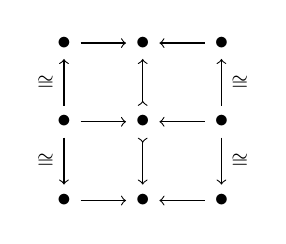
\begin{tikzpicture}
  \node (00) at (0,0) {$ \bullet $};
  \node (01) at (0,1) {$ \bullet $};
  \node (02) at (0,2) {$ \bullet $};
  \node (10) at (1,0) {$ \bullet $};
  \node (11) at (1,1) {$ \bullet $};
  \node (12) at (1,2) {$ \bullet $};
  \node (20) at (2,0) {$ \bullet $};
  \node (21) at (2,1) {$ \bullet $};
  \node (22) at (2,2) {$ \bullet $};
  \draw [->] (02) to node [] {\scriptsize{$  $}} (12);
  \draw [->] (22) to node [] {\scriptsize{$  $}} (12);
  \draw [->] (01) to node [] {\scriptsize{$  $}} (11);
  \draw [->] (21) to node [] {\scriptsize{$  $}} (11);
  \draw [->] (00) to node [] {\scriptsize{$  $}} (10);
  \draw [->] (20) to node [] {\scriptsize{$  $}} (10);
  \draw [->] (01) to node [left] {\scriptsize{$ \cong  $}} (02);
  \draw [->] (01) to node [left] {\scriptsize{$ \cong $}} (00);
  \draw [>->] (11) to node [] {\scriptsize{$  $}} (12);
  \draw [>->] (11) to node [] {\scriptsize{$  $}} (10);
  \draw [->] (21) to node [right] {\scriptsize{$ \cong $}} (22);
  \draw [->] (21) to node [right] {\scriptsize{$ \cong $}} (20);
\end{tikzpicture}
\]
%

Given a structured cospan grammar $ ( _{L}\StrCsp , P ) $,
observe that the productions in $ P $ are admissible as
squares in $ \MonSpCsp (\X) $. Denote by
$ S ( _{L}\StrCsp , P ) $ the sub-double category of
$ \MonSpCsp ( \X ) $ that is full on objects, vertical and
horizontal arrows, and generated by the rules in
$ P $. This assignment is functorial because
\[
  (F,G) \from ( _{L}\StrCsp , P ) \to ( StrCsp , P )
\]
gives a mapping between the generators of
$ S ( _{L}\StrCsp , P ) $ and $ S ( _{L'}\StrCsp , P' ) $.
Composition holds because $ F $ and $ G $ both preserve
pullbacks and pushouts. This allows us to define the
language functor $ \Lang \coloneqq SD $.

